\documentclass[12pt]{article}
\usepackage{amsfonts,amssymb,float,amsmath}
\usepackage{algorithmic}
\usepackage{graphicx, siunintx}
\usepackage{textcomp}
\usepackage{xcolor}
\usepackage{txfonts}
\usepackage{multicol}
\usepackage{listings}
\usepackage{enumitem}
\usepackage{mathtools}
\usepackage{gensymb}
\usepackage{comment}
\usepackage[breaklinks=true]{hyperref}
\usepackage{tkz-euclide} 
\usepackage{listings}
\usepackage{gvv}                       
\usepackage{gvv-book}
%\def\inputGnumericTable{}                             
\usepackage{color}                                            
\usepackage{array}                                            
\usepackage{longtable}                                       
\usepackage{calc}                                             
\usepackage{multirow}                                         
\usepackage{hhline}                                           
\usepackage{ifthen}                                           
\usepackage{lscape}
\newcommand{\BEQA}{\begin{eqnarray}}
\newcommand{\EEQA}{\end{eqnarray}}
%\newcommand{\define}{\stackrel{\triangle}{=}}
\theoremstyle{remark}
\newtheorem{rem}{Remark}
\parindent 0px
\pagenumbering{gobble}
\begin{document}
\title{\vspace{-5cm}Gate paper 2023-XH}
\author{Ayush Sunil Labhade}
\date{AI25Btech11002}
\maketitle

\begin{flushright}Humanities and Social Sciences – Psychology (XH-C5)\end{flushright}
\begin{flushleft}General Aptitude \textbf{\brak{GA}} \\[5pt]
\textbf{\item Q.1 – Q.5 Carry ONE mark Each}\end{flushleft}
\begin{enumerate}
%Q.1
\item Rafi told Mary, “I am thinking of watching a film this weekend.”
The following reports the above statement in indirect speech: 
Rafi told Mary that he \_\_\_\_\_\_\_ of watching a film that weekend.
\begin{enumerate}
    \begin{multicols}{2}
        \item thought
        \item is thinking
        \item am thinking
        \item was thinking
    \end{multicols}
\end{enumerate}
\hfill\brak{GATE \ XH \ 2023}
%Q.2
\item Permit : \_\_\_\_\_\_\_ : : Enforce : Relax 
\brak{By word meaning}
\begin{enumerate}
    \begin{multicols}{4}
        \item Allow
        \item Forbid
        \item License
        \item Reinforce
    \end{multicols}
\end{enumerate}
\hfill\brak{GATE \ XH \ 2023}
%Q.3
\item Given a fair six-faced dice where the faces are labelled ‘1’, ‘2’, ‘3’, ‘4’, ‘5’, and ‘6’, 
what is the probability of getting a ‘1’ on the first roll of the dice and a ‘4’ on the 
second roll?
\begin{enumerate}
    \begin{multicols}{4}
        \item $\frac{1}{36}$
        \item $\frac{1}{6}$
        \item $\frac{5}{6}$
        \item $\frac{1}{3}$
    \end{multicols}
\end{enumerate}
\hfill\brak{GATE \ XH \ 2023}
%Q.4
\item A recent survey shows that 65% of tobacco users were advised to stop consuming tobacco.
The survey also shows that 3 out of 10 tobacco users attempted to stop using tobacco.
Based only on the information in the above passage, which one of the following options can be logically inferred with certainty?
\begin{enumerate}
    \item A majority of tobacco users who were advised to stop consuming tobacco made an attempt to do so.
    \item A majority of tobacco users who were advised to stop consuming tobacco did not attempt to do so.
    \item Approximately 30% of tobacco users successfully stopped consuming tobacco.
    \item Approximately 65% of tobacco users successfully stopped consuming tobacco.
\end{enumerate}
\hfill\brak{GATE \ XH \ 2023}
%Q.5
\item How many triangles are present in the given figure?
\begin{figure}[H]
    \centering
    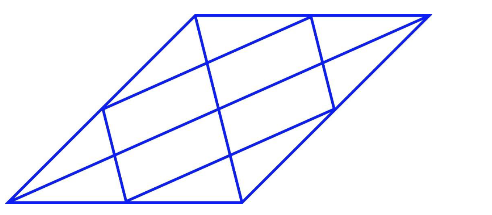
\includegraphics[width=0.5\textwidth]{Figs/Q5.png}
    \caption{}
    \label{fig:5.1}
\end{figure}
\begin{enumerate}
    \begin{multicols}{4}
        \item 12
        \item 16
        \item 20
        \item 24
    \end{multicols}
\end{enumerate}
\hfill\brak{GATE \ XH \ 2023}
\newpage
\textbf{Q.6 – Q.10 Carry TWO marks Each}
%Q.6
\item Students of all the departments of a college who have successfully completed the registration process are eligible to vote in the upcoming college elections. However, by the time the due date for registration was over, it was found that surprisingly none of the students from the Department of Human Sciences had completed the registration process. Based only on the information provided above, which one of the following sets of statement(s) can be logically inferred with certainty?
\begin{enumerate}
    \item[(i)] All those students who would not be eligible to vote in the college elections would certainly belong to the Department of Human Sciences.
    \item[(ii)] None of the students from departments other than Human Sciences failed to complete the registration process within the due time.
    \item[(iii)] All the eligible voters would certainly be students who are not from the Department of Human Sciences.
\end{enumerate}
\begin{enumerate}
    \begin{multicols}{4}
        \item (i) and (ii)
        \item (i) and (iii)
        \item only (i)
        \item only (iii)
    \end{multicols}
\end{enumerate}
\hfill\brak{GATE \ XH \ 2023}
%Q.7
\item Which one of the following options represents the given graph?
\begin{figure}[H]
    \centering
    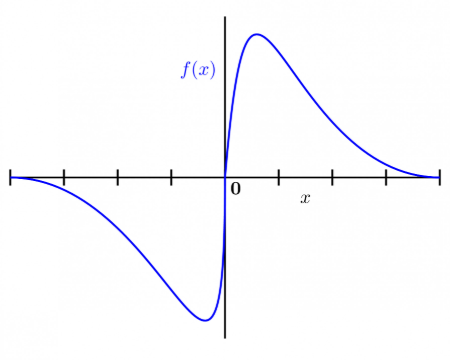
\includegraphics[width=0.6\textwidth]{Figs/Q7.png}
    \caption{}
    \label{fig:5.2}
\end{figure}
\begin{enumerate}
    \begin{multicols}{4}
        \item $f(x)=x^22^{-|x|}$ 
        \item $f(x)=x2^{-|x|}$
        \item $f(x)=|x|2^{-x}$ 
        \item $f(x)=x2^{-x}$
    \end{multicols}
\end{enumerate}
\hfill\brak{GATE \ XH \ 2023}
%Q.8
\item Which one of the options does NOT describe the passage below or follow from it?
We tend to think of cancer as a ‘modern’ illness because its metaphors are so modern. It is a disease of overproduction, of sudden growth, a growth that is unstoppable, tipped into the abyss of no control. Modern cell biology encourages us to imagine the cell as a molecular machine. Cancer is that machine unable to quench its initial command \brak{to grow} and thus transform into an indestructible, self-propelled automaton.
\sbrak{Adapted from \textit{The Emperor of All Maladies} by Siddhartha Mukherjee}
\begin{enumerate}
    \item It is a reflection of why cancer seems so modern to most of us.
    \item It tells us that modern cell biology uses and promotes metaphors of machinery.
    \item Modern cell biology encourages metaphors of machinery, and cancer is often imagined as a machine.
    \item Modern cell biology never uses figurative language, such as metaphors, to describe or explain anything.
\end{enumerate}
\hfill\brak{GATE \ XH \ 2023}
%Q.9
\item The digit in the unit’s place of the product $3^{999} \times 7^{1000}$ is \_\_\_\_\_\_\_.
\begin{enumerate}
    \begin{multicols}{4}
        \item 7
        \item 1
        \item 3
        \item 9
    \end{multicols}
\end{enumerate}
\hfill\brak{GATE \ XH \ 2023}
%Q.10
\item A square with sides of length 6 cm is given. The boundary of the shaded region is defined by two semi-circles whose diameters are the sides of the square, as shown. The area of the shaded region is \_\_\_\_\_\_\_ cm$^2$.
\begin{figure}[H]
    \centering
    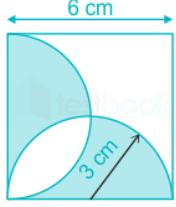
\includegraphics[width=0.3\textwidth]{Figs/Q10.png}
    \caption{}
    \label{fig:5.3}
\end{figure}
\begin{enumerate}
    \begin{multicols}{4}
        \item $6\pi$
        \item 18
        \item 20
        \item $9\pi$
    \end{multicols}
\end{enumerate}
\hfill\brak{GATE \ XH \ 2023}
\newpage
\textbf{Reasoning and Comprehension (XH-B1)\newline XH-B1: Q.11 – Q.17 Carry ONE mark Each}
%Q.11
\item Which word below best describes the idea of being both Spineless and Cowardly?
\begin{enumerate}
    \begin{multicols}{2}
        \item Pusillanimous
        \item Unctuous
        \item Obsequious
        \item Reticent
    \end{multicols}
\end{enumerate}
\hfill\brak{GATE \ XH \ 2023}
%Q.12
\item Choose the right preposition to fill up the blank: The whole family got together \_\_\_\_\_\_\_ Diwali
\begin{enumerate}
    \begin{multicols}{4}
        \item of
        \item at
        \item in
        \item till
    \end{multicols}
\end{enumerate}
\hfill\brak{GATE \ XH \ 2023}
%Q.13
\item Select the correct option to fill in all the blanks to complete the passage:
The (i)\_\_\_\_\_\_\_ factor amid this turbulence has been the (ii)\_\_\_\_\_\_\_\_ of high
octane, action-oriented films such as RRR, K.G.F: Chapter 2 and Pushpa from film
industries in the south of the country. Traditionally, films made in the south have
done well in their own (iii) \_\_\_\_\_\_\_\_\_. But increasingly, their dubbed versions
have performed well in the Hindi heartland, with collections (iv)\_\_\_\_\_\_\_\_ those of
their Bollywood counterparts.
\begin{enumerate} 
\item (i) disheartening (ii) failure (iii) channels (iv) matching
\item (i) redeeming (ii) outperformance (iii) geographies (iv) eclipsing
\item (i) shocking (ii) underperformance (iii) cinemas (iv) below
\item (i) humbling (ii) bombing (iii) theatres (iv) falling behind
\end{enumerate}
\hfill\brak{GATE \ XH \ 2023}
%Q.14
\item The following passage consists of 6 sentences. The first and sixth sentences of the
passage are at their correct positions, while the middle four sentences (represented
by 2, 3, 4, and 5) are jumbled up. Choose the correct sequence of the sentences so that they form a coherent
paragraph:
\begin{enumerate}
\item[1.] Most obviously, mobility is taken to be a geographical as well as a social phenomenon.
\item[2.] Much of the social mobility literature regarded society as a uniform surface and failed to register the geographical intersections of region, city and place, with the social categories of class, gender and ethnicity.
\item[3.] The existing sociology of migration is incidentally far too limited in its concerns to be very useful here.
\item[4.] Further, I am concerned with the flows of people within, but especially beyond, the territory of each society, and how these flows may relate to many different desires, for work, housing, leisure, religion, family relationships, criminal gain, asylum seeking and so on.
\item[5.] Moreover, not only people are mobile but so too are many ‘objects’.
\item[6.] I show that sociology’s recent development of a ‘sociology of objects’ needs to be taken further and that the diverse flows of objects across societal borders and their intersections with the multiple flows of people are hugely significant.
\end{enumerate}
\begin{enumerate}
    \begin{multicols}{4}
        \item 3, 2, 5, 4
        \item 2, 3, 4, 5
        \item 5, 4, 3, 2
        \item 4, 2, 5, 3
    \end{multicols}
\end{enumerate}
\hfill\brak{GATE \ XH \ 2023}
%Q.15
\item The population of a country increased by 5\% from 2020 to 2021. Then, the
population decreased by 5\% from 2021 to 2022. By what percentage did the
population change from 2020 to 2022?
\begin{enumerate}
    \begin{multicols}{4}
        \item -0.25\%
        \item 0\%
        \item 2.5\%
        \item 10.25\%
    \end{multicols}
\end{enumerate}
\hfill\brak{GATE \ XH \ 2023}
%Q.16
\item The words \textbf{Thin: Slim: Slender} are related in some way.
Identify the correct option(s) that reflect(s) the same relationship:
\begin{enumerate}
    \begin{multicols}{2}
        \item Fat: Plump: Voluptuous
        \item Short: Small: Petite
        \item Tall: Taller: Tallest
        \item Fair: Dark: Wheatish
    \end{multicols}
\end{enumerate}
\hfill\brak{GATE \ XH \ 2023}
%Q.17
\item A pandemic like situation hit the country last year, resulting in loss of human life and economic depression. To improve the condition of its citizens, the government made a series of emergency medical interventions and increased spending to revive the economy. In both these efforts, district administration authorities were actively involved. Which of the following action(s) are plausible?
\begin{enumerate}
    \item In future, the government can make district administration authorities responsible for protecting health of citizens and reviving the economy.
    \item The government may set up a task force to review the post pandemic situation and ascertain the effectiveness of the measures taken.
    \item The government may set up a committee to formulate a pandemic management program to minimize losses to life and economy in future.
    \item The government may take population control measures to minimize pandemic related losses in future.
\end{enumerate}
\hfill\brak{GATE \ XH \ 2023}
\newpage
\textbf{XH-B1: Q.18 – Q.26 Carry TWO marks Each}
%Q.18
\item Six students, Arif, Balwinder, Chintu, David, Emon and Fulmoni appeared in the GATE-XH exam in 2022. Balwinder scores less than Chintu in XH-B1, but more than Arif in XH-C1. David scores more than Balwinder in XH-C1, and more than Chintu in XH-B1. Emon scores less than David, but more than Fulmoni in XH-B1. Fulmoni scores more than David in XH-C1. Arif scores less than Emon, but more than Fulmoni in XH-B1. Who scores highest in XH-B1?
\begin{enumerate}
    \begin{multicols}{4}
        \item Fulmoni
        \item Emon
        \item David
        \item Chintu
    \end{multicols}
\end{enumerate}
\hfill\brak{GATE \ XH \ 2023}
%Q.19
\item Select the correct relation between E and F.
$$ E = \frac{x}{1+x} \quad \text{and} \quad F = \frac{-x}{1-x} \quad x > 1 $$
\begin{enumerate}
    \begin{multicols}{4}
        \item E $>$ F
        \item E $<$ F
        \item E $=$ F
        \item E $<$ -F
    \end{multicols}
\end{enumerate}
\hfill\brak{GATE \ XH \ 2023}
%Q.20
\item A code language is formulated thus:
Vowels in the original word are replaced by the next vowel from the list of vowels, A-E-I-O-U \brak{For example, E is replaced by I and U is replaced by A}. Consonants in the original word are replaced by previous consonant \brak{For example, T is replaced by S and V is replaced by T}. Then how does the word, GOODMORNING appear in the coded language?
\begin{enumerate}
    \begin{multicols}{2}
        \item HUUFNUSPOPH
        \item FIICLIQMEMF
        \item FUUCLUQMOMF
        \item HEEDATTACRH
    \end{multicols}
\end{enumerate}
\hfill\brak{GATE \ XH \ 2023}
%Q.21
\item The stranger is by nature no "owner of soil" -- soil not only in the physical, but also in the figurative sense of a life-substance, which is fixed, if not in a point in space, at least in an ideal point of the social environment. Although in more intimate relations, he may develop all kinds of charm and significance, as long as he is considered a stranger in the eyes of the other, he is not an "owner of soil." Restriction to intermediary trade, and often \brak{as though sublimated from it} to pure finance, gives him the specific character of mobility. If mobility takes place within a closed group, it embodies that synthesis of nearness and distance which constitutes the formal position of the stranger. For, the fundamentally mobile person comes in contact, at one time or another, with every individual, but is not organically connected, through established ties of kinship, locality, and occupation, with any single one. What assumptions can be made about the stranger from the passage above?
\begin{enumerate}
    \item The stranger can become an owner of soil through developing all kinds of charm in more intimate relations.
    \item The stranger cannot become an owner of soil either in the physical or psychological sense.
    \item The stranger can become an owner of soil through establishing ties of kinship and so on.
    \item The stranger might become an owner of soil in the physical sense but not in the psychological
\end{enumerate}
\hfill\brak{GATE \ XH \ 2023}
%Q.22
\item L is the only son of A and S. S has one sibling, B, who is married to L’s aunt, K. B is the only son of D. How are L and D related? Select the possible option(s):
\begin{enumerate}
    \item Grandchild and Paternal Grandfather
    \item Grandchild and Maternal Grandfather
    \item Grandchild and Paternal Grandmother
    \item Grandchild and Maternal Grandmother
\end{enumerate}
\hfill\brak{GATE \ XH \ 2023}
%Q.23
\item Five segments of a sentence are given below. The first and fifth segments are at their correct positions, while the middle three segments \brak{represented by 2, 3, and 4} are jumbled up. Choose the correct order of the segments so that they form a coherent sentence:
\begin{enumerate}
    \item[1.] Consumed multitudes are jostling and shoving inside me
    \item[2.] and guided only by the memory of a large white bedsheet with a roughly circular hole some seven inches in diameter cut into the center, 
    \item[3.] clutching at the dream of that holey, mutilated square of linen, which is my talisman, my open-sesame,
    \item[4.] I must commence the business of remaking my life from the point at which it really began, 
    \item[5.] some thirty-two years before anything as obvious, as present, as my clock-ridden, crime-stained birth. 
\end{enumerate}
\begin{enumerate}
    \begin{multicols}{4}
        \item 2 – 3 – 4
        \item 3 – 2– 4
        \item 4 – 2– 3
        \item 4 – 3 – 2
    \end{multicols}
\end{enumerate}
\hfill\brak{GATE \ XH \ 2023}
%Q.24
\item “I told you the truth,” I say yet again, “Memory’s truth, because memory has its own special kind. It selects, eliminates, alters, exaggerates, minimizes, glorifies, and vilifies also; but in the end it creates its own reality, its heterogeneous but usually coherent versions of events; and no sane human being ever trusts someone else’s version more than his own.” What are the different ways in which ‘truth’ can be understood from the passage?
\begin{enumerate}
    \item Truth is what can be verified by hard empirical evidence.
    \item Truth is based on what can be perceived by the senses.
    \item Truth is the product of memory that is fallible, selective and slanted.
    \item Truth is contingent on the observer and can only be partial.
\end{enumerate}
\hfill\brak{GATE \ XH \ 2023}
%Q.25
\item A firm needs both skilled labour and unskilled labour for the production of cloth. The wage of skilled labour is Rs. 40,000 per month, and that of unskilled labour is Rs. 15,000 per month. The total wage bill of the firm for the production of cloth is Rs. 23,75,000 in a month for 100 labour. How many skilled labour are employed by the firm \brak{in Integer}?
\hfill\brak{GATE \ XH \ 2023}
%Q.26
\item Select the odd word and write the option number as answer: (1) Lek (2) Zloty (3) Diner (4) Drachma (5) Real
\hfill\brak{GATE \ XH \ 2023}
\newpage
\textbf{Psychology – C5\newline XH-C5: Q.27 – Q.44 Carry ONE mark Each}
%Q.27
\item Blind spot in the retina contains\_\_\_\_\_\_\_\_\_\_\_\_\_\_\_\_\_\_\_\_\_\_\_\_\_\_\_\_\_\_\_\_\_\_\_\_\_\_\_\_.
	\begin{enumerate} \begin{multicols}{2}
    \item only rod cells
    \item only cone cells
    \item both rod and cone cells
    \item neither rod nor cone cells
	\end{multicols} \end{enumerate}
\hfill\brak{GATE \ XH \ 2023}
%Q.28
\item Taking painkillers eliminates pain, increasing the likelihood that the person will take painkillers again. This is an example of\_\_\_\_\_\_\_\_\_\_\_\_\_\_\_\_\_\_\_\_\_\_\_\_\_\_\_\_.
	\begin{enumerate} \begin{multicols}{2}
    \item negative punishment
    \item positive reinforcement
    \item negative reinforcement
    \item positive punishment
	\end{multicols} \end{enumerate}
\hfill\brak{GATE \ XH \ 2023}
%Q.29
\item When learning something new impairs the ability to retrieve information learnt earlier, it is known as \_\_\_\_\_\_\_\_\_\_\_\_\_\_\_\_\_\_\_\_\_\_.
	\begin{enumerate} \begin{multicols}{2}
    \item retroactive interference
    \item proactive interference 
    \item tip-of-the-tongue phenomenon
    \item recency effect 
	\end{multicols} \end{enumerate}
\hfill\brak{GATE \ XH \ 2023}
%Q.30
\item Iconic memory is a type of \_\_\_\_\_\_\_\_\_\_\_\_\_\_\_\_.
\begin{enumerate}
    \begin{multicols}{2}
        \item short term memory
        \item sensory memory
        \item semantic memory
        \item working memory
    \end{multicols}
\end{enumerate}
\hfill\brak{GATE \ XH \ 2023}
%Q.31
\item Which one of the following components of language has to do with the practical or social aspects of communication with others?
\begin{enumerate}
    \begin{multicols}{4}
        \item Phonemes
        \item Morphemes
        \item Pragmatics
        \item Syntax
    \end{multicols}
\end{enumerate}
\hfill\brak{GATE \ XH \ 2023}
%Q.32
\item The Yerkes-Dodson law states that\_\_\_\_\_\_\_\_\_\_\_\_\_\_\_\_\_\_\_\_\_\_\_\_\_\_\_\_\_\_\_\_\_\_\_.
\begin{enumerate}
    \item performance is affected by the level of arousal
    \item frustration leads to aggression
    \item self-concept helps us organize and remember information
    \item changes in behaviour are a result of experiences that have happened frequently or recently
\end{enumerate}
\hfill\brak{GATE \ XH \ 2023}
%Q.33
\item Transduction of mechanical energy into nerve impulses in the auditory system takes place in reponse to bending of the\_\_\_\_\_\_\_\_\_\_\_\_\_\_\_\_.
\begin{enumerate}
    \begin{multicols}{4}
        \item pinna
        \item hair cells
        \item incus
        \item malleus
    \end{multicols}
\end{enumerate}
\hfill\brak{GATE \ XH \ 2023}
%Q.34
\item Which one of the following theories states that emotion occurs as a result of physical arousal and labeling of the arousal based on cues from the surrounding environment?
\begin{enumerate}
    \begin{multicols}{2}
        \item Ekman-Friesen theory
        \item Schachter-Singer theory
        \item James-Lange theory
        \item Cannon-Bard theory
    \end{multicols}
\end{enumerate}
\hfill\brak{GATE \ XH \ 2023}
%Q.35
\item Which one of the following is TRUE for the Pain-Gate control theory?
\begin{enumerate}
    \item Gate is a physical structure
    \item Activity of gate cannot be closed by non-pain signals
    \item Substance P released into spinal cord does not activate other neurons that send messages through spinal gates
    \item Pain signals must pass through a gate located in the spinal cord
\end{enumerate}
\hfill\brak{GATE \ XH \ 2023}
%Q.36
\item Being treated with warmth and consideration by others only when one behaves as expected, is called as\_\_\_\_\_\_\_\_\_\_\_\_\_\_\_\_\_\_\_\_\_\_\_\_\_\_\_\_\_\_\_\_\_\_\_\_\_\_\_\_.
	\begin{enumerate} \begin{multicols}{2}
    \item openness to experience
    \item conditional positive regard 
    \item unconditional positive regard
    \item zone of proximal development
	\end{multicols} \end{enumerate}
\hfill\brak{GATE \ XH \ 2023}
%Q.37
\item Which of the following is/are NOT the factor(s) of the Big Five Personality model?
	\begin{enumerate} \begin{multicols}{2}
    \item Conscientiousness
    \item Optimism 
    \item Humility
    \item Extraversion
	\end{multicols} \end{enumerate}
\hfill\brak{GATE \ XH \ 2023}
%Q.38
\item Which of the following is/are TRUE for creative individuals?
\begin{enumerate}
    \item They are not very good at mental imagery
    \item They are not afraid to be different
    \item They do not value their independence 
    \item They are unconventional in their work
\end{enumerate}
\hfill\brak{GATE \ XH \ 2023}
%Q.39
\item Which of the following is/are included under behavioural genetics studies in humans?
	\begin{enumerate} \begin{multicols}{2}
    \item Selective breeding studies
    \item Family studies
    \item Twin studies
    \item Adoption studies
	\end{multicols} \end{enumerate}
\hfill\brak{GATE \ XH \ 2023}
%Q.40
\item Which of the following statements regarding locus of control is/are CORRECT?
\begin{enumerate}
    \item It can be internal and/or external
    \item It is associated with self-esteem
    \item Internal locus of control is positively correlated with success
    \item Regret has no association with locus of control
\end{enumerate}
\hfill\brak{GATE \ XH \ 2023}
%Q.41
\item Which of the following is/are TRUE for nonparametric statistics?
\begin{enumerate}
    \item It is often called distribution free statitstics
    \item It is used to analyze interval data
    \item It is used to analyze ordinal data
    \item It compares groups in terms of means
\end{enumerate}
\hfill\brak{GATE \ XH \ 2023}
%Q.42
\item According to the review of research on stress and immune system, which of the following statement(s) has/have substantial evidence?
\begin{enumerate}
    \item There is a negative relationship between stress and functional immune measures
    \item There is no measurable impact of stress on functional immune measures
    \item Loneliness impacts the relationship between stress and functional immune measures  
    \item There is a positive relationship between long term stressors and functional immune measures
\end{enumerate}
\hfill\brak{GATE \ XH \ 2023}
%Q.43
\item Which of the following influence(s) gender dysphoria?
\begin{enumerate}
    \item Prenatal factors
    \item Early childhood experiences
    \item Socialization
    \item Attention Deficit Hyperactivity Disorder
\end{enumerate}
\hfill\brak{GATE \ XH \ 2023}
%Q.44
\item If the variance of a set of scores is 100, the standard deviation is\_\_\_\_\_\_ \brak{in integer}.
\hfill\brak{GATE \ XH \ 2023}
\newpage
\textbf{XH-C5: Q.45– Q.65 Carry TWO marks Each}
%Q.45
\item Match the structures of the brain in the first column with their respective functions in the second column of the table given below.
\begin{table}[H]
    \centering
     \begin{tabular}{|l|p{7cm}|}
        \hline
        \textbf{Brain Structures} & \textbf{Functions} \\
        \hline
        P) Cerebellum & i) Orients a person in the environment \\
        Q) Thalamus & ii) Coordinates heart rate, circulation, and respiration \\
        R) Tectum & iii) Controls fine motor skills \\
        S) Medulla & iv) Relays and filters information from the senses and transmits the information to the cerebral cortex \\
        \hline
    \end{tabular}


    \caption{}
    \label{tab:5.1}
\end{table}
\begin{enumerate} \begin{multicols}{2}
    \item P-(iii), Q-(i), R-(iv), S-(ii)
    \item P-(i), Q-(iv), R-(ii), S-(iii)
    \item P-(iv), Q-(iii), R-(ii), S-(i)
    \item P-(iii), Q-(iv), R-(i), S-(ii)
\end{multicols} \end{enumerate}
\hfill\brak{GATE \ XH \ 2023}
%Q.46
\item Which one of the following is established by the replication of research studies?
\begin{enumerate}
    \begin{multicols}{2}
        \item Validity of the results
        \item Reliability of the results
        \item Interaction effect
        \item Mediation effect
    \end{multicols}
\end{enumerate}
\hfill\brak{GATE \ XH \ 2023}
%Q.47
\item Match the theory/law in the first column with the corresponding explanation in the second column of the table given below.
\begin{table}[H]
    \centering
     \begin{tabular}{|l|p{7cm}|}
        \hline
        \textbf{Theory/law} & \textbf{Explanation} \\
        \hline
        P) Weber’s law & i) The detection of change in a stimulus is relative to the magnitude of the stimulus \\
        Q) Steven’s Power law & ii) Sensory magnitude grows in proportion to the physical intensity of the stimulus raised to a power \\
        R) Signal detection theory & iii) The magnitude of a sensation is a logarithmic function of the stimulus \\
        S) Fechner’s law & iv) The ability to detect a weak stimulus varies from moment to moment as per response bias \\
        \hline
    \end{tabular}


    \caption{}
    \label{tab:5.2}
\end{table}
\begin{enumerate} \begin{multicols}{2}
    \item P-(ii), Q-(iv), R-(i), S-(iii)
    \item P-(iv), Q-(iii), R-(ii), S-(i)
    \item P-(i), Q-(ii), R-(iv), S-(iii)
    \item P-(iii), Q-(ii), R-(iv), S-(i)
\end{multicols} \end{enumerate}
\hfill\brak{GATE \ XH \ 2023}
%Q.48
\item Match the sleep disorders in the first column with the symptoms in the second column of the table given below.
\begin{table}[H]
    \centering
     \begin{tabular}{|l|p{7cm}|}
        \hline
        \textbf{Sleep disorders} & \textbf{Symptoms} \\
        \hline
        P) Enuresis & i) Excessive daytime sleepiness \\
        Q) Hypersomnia & ii) Urinating while asleep in bed \\
        R) Circadian rhythm disorder & iii) A disorder in which the person stops breathing for brief periods while asleep \\
        S) Sleep apnea & iv) Disturbances of the sleep-wake cycle \\
        \hline
    \end{tabular}


    \caption{}
    \label{tab:5.3}
\end{table}
\begin{enumerate} \begin{multicols}{2}
    \item P-(ii), Q-(iv), R-(i), S-(iii)
    \item P-(ii), Q-(i), R-(iv), S-(iii)
    \item P-(ii), Q-(i), R-(iii), S-(iv)
    \item P-(iii), Q-(iv), R-(i), S-(ii)
	    \end{multicols} \end{enumerate}
\hfill\brak{GATE \ XH \ 2023}
%Q.49
\item \_\_\_\_\_\_\_\_\_\_\_\_\_\_\_\_\_\_\_\_\_\_ explains aging as a process of mutual withdrawal of individual and society, whereas \_\_\_\_\_\_\_\_\_\_\_\_\_\_\_\_\_\_\_\_\_\_ assumes positive correlation between activity and successful aging.
\begin{enumerate}
    \item Decay theory, Engagement theory
    \item Balance theory, Engagement theory
    \item Disengagement theory, Activity theory
    \item Withdrawal theory, Activity theory
\end{enumerate}
\hfill\brak{GATE \ XH \ 2023}
%Q.50
\item Match the biases/effects in the first column with the descriptions in the second column of the table given below.
\begin{table}[H]
    \centering
     \begin{tabular}{|l|p{7cm}|}
        \hline
        \textbf{Biases/effects} & \textbf{Descriptions} \\
        \hline
        P) Barnum Effect & i) Tendency to take credit for one’s success but downplaying responsibility for one’s failure \\
        Q) Reference Group Effect & ii) Tendency to take blame for failure but downplay one’s role in the success \\
        R) Self-Serving Bias & iii) Tendency to rate oneself with repect to one’s social and cultural group \\
        S) Self-Effacing Bias & iv) Tendency to believe in description of personality that is supposedly descriptive of oneself, but could in fact describe almost anyone \\
        \hline
    \end{tabular}


    \caption{}
    \label{tab:5.4}
\end{table}
\begin{enumerate} \begin{multicols}{2}
    \item P-(i), Q-(iii), R-(ii), S-(iv)
    \item P-(iv), Q-(iii), R-(i), S-(ii)
    \item P-(iv), Q-(iii), R-(ii), S-(i)
    \item P-(iv), Q-(i), R-(ii), S-(iii)
\end{multicols} \end{enumerate}
\hfill\brak{GATE \ XH \ 2023}
%Q.51
\item Match the theories in the first column with the central themes in the second column of the table given below.
\begin{table}[H]
    \centering
     \begin{tabular}{|l|p{7cm}|}
        \hline
        \textbf{Theories} & \textbf{Central themes} \\
        \hline
        P) Drive theory & i) Our general level of activation leads to optimization \\
        Q) Arousal theory & ii) Behaviour is determined by desirable outcomes \\
        R) Expectancy theory & iii) Setting specific and challenging goals boosts motivation \\
        S) Goal setting theory & iv) Biological needs push us to action \\
        \hline
    \end{tabular}


       \caption{}
    \label{tab:5.5}
\end{table}
\begin{enumerate} \begin{multicols}{2}
    \item P-(iv), Q-(i), R-(ii), S-(iii)
    \item P-(iv), Q-(i), R-(iii), S-(ii)
    \item P-(i), Q-(iv), R-(ii), S-(iii)
    \item P-(ii), Q-(iii), R-(i), S-(iv)
\end{multicols} \end{enumerate}
\hfill\brak{GATE \ XH \ 2023}
%Q.52
\item Which one of the following would resolve the basic dilemma of the social psychologist?
\begin{enumerate}
    \item Conducting carefully designed experiments with high internal validity
    \item By replicating experiments and conducting some new experiments that have internal validity and others that have external validity
    \item Conducting research exclusively in the field
    \item Conducting applied rather than basic research
\end{enumerate}
\hfill\brak{GATE \ XH \ 2023}
%Q.53
\item Match the research methods in the first column with their purposes in the second column of the table given below.
\begin{table}[H]
    \centering
        \begin{tabular}{|l|p{6cm}|}
        \hline
        \textbf{Research Methods} & \textbf{Purposes} \\
        \hline
        P) Narrative method & i) Describing a person, event, and experience in detail \\
        Q) Ethnography & ii) Collecting data in the form of cohesive stories \\
        R) Case Study & iii) Extracting themes from data \\
        S) Content analysis & iv) Describing cultural characteristics in detail \\
        \hline
    \end{tabular}


    \caption{}
    \label{table:5.6}
\end{table}
\begin{enumerate} \begin{multicols}{2}
    \item P-(i), Q-(iii), R-(ii), S-(iv)
    \item P-(ii), Q-(iii), R-(iv), S-(i)
    \item P-(i), Q-(iv), R-(ii), S-(iii)
    \item P-(ii), Q-(iv), R-(i), S-(iii)
\end{multicols} \end{enumerate}
\hfill\brak{GATE \ XH \ 2023}
%Q.54
\item Which one of the following statements is TRUE according to Brehm’s reactance theory?
\begin{enumerate}
    \item A mild sign prohibitting spitting would be more effective in preventing spitting than a strong sign
    \item A strong sign would be more effective in preventing spitting than a mild one
    \item Absence of any sign would be most effective in preventing spitting
    \item Signs are irrelevant to spitting behaviour
\end{enumerate}
\hfill\brak{GATE \ XH \ 2023}
%Q.55
\item According to the overjustifcation effect, which one of the following consequences would be TRUE for students who freely choose to study psychology, if marks are given for attendance?
\begin{enumerate}
    \item Increased interest of students in the subject
    \item Decreased interest of students in the subject
    \item No effect on the interest of students in the subject
    \item Increased interest in other social science subjects
\end{enumerate}
\hfill\brak{GATE \ XH \ 2023}
%Q.56
\item Large rewards and severe punishments are examples of \_\_\_\_\_\_\_\_\_\_\_\_\_\_\_ justification for behaviour and result in\_\_\_\_\_\_\_\_\_\_\_\_ changes in attitude.
\begin{enumerate}
    \item internal; big
    \item external; big
    \item internal; small
    \item external; small
\end{enumerate}
\hfill\brak{GATE \ XH \ 2023}
%Q.57
\item Which of the following therapies is/are based on classical conditioning?
\begin{enumerate}
    \item Systematic desensitization
    \item Aversion therapy
    \item Cognitive behaviour therapy
    \item Rational emotive behaviour therapy
\end{enumerate}
\hfill\brak{GATE \ XH \ 2023}
%Q.58
\item Which of the following characterize(s) Wernicke’s aphasia?
\begin{enumerate}
    \item Inability to comprehend spoken words
    \item Inability to understand the meaning of words
    \item Inability to speak grammatically correct language
    \item Inability to write and understand the symbols that represent speech sounds
\end{enumerate}
\hfill\brak{GATE \ XH \ 2023}
%Q.59
\item Which of the following is/are the component(s) of Theory of Mind?
\begin{enumerate}
    \item Understanding that people can have false beliefs
    \item Distinguishing faces and smells
    \item Recognizing that others have mental states
    \item Having a vast vocabulary to express one’s thoughts
\end{enumerate}
\hfill\brak{GATE \ XH \ 2023}
%Q.60
\item Which of the following would NOT be effective in minimizing groupthink?
\begin{enumerate}
    \item The leader being impartial to all ideas no matter what they are
    \item The leader reminding the team that everyone will be held responsible for the decision of the group
    \item The leader taking all decisions on behalf of the group
    \item The leader arriving at a consensus quickly
\end{enumerate}
\hfill\brak{GATE \ XH \ 2023}
%Q.61
\item Which of the following describe(s) the standard error of the mean?
\begin{enumerate}
    \item It is the standard deviation of the sampling distribution of the mean
    \item It reflects the accuracy with which sample means estimate the population mean
    \item It is the difference between mean and standard deviation of a distribution 
    \item It is the standard deviation of a stratified sample
\end{enumerate}
\hfill\brak{GATE \ XH \ 2023}
%Q.62
\item Which of the following describe(s) organizational commitment?
\begin{enumerate}
    \item A strong desire to remain a member of the organization
    \item Willingness to exert high level of effort on behalf of the organization
    \item A definite belief in and acceptance of values and goals of the organization
    \item High turnover intention of the employees of the organization 
\end{enumerate}
\hfill\brak{GATE \ XH \ 2023}
%Q.63
\item Prejudice is supported by the human tendency to categorize into in-groups and out-groups. Prejudice is supported by which of the following processes?
\begin{enumerate}
    \item The way we think about others
    \item The way we assign meaning to others behaviour
    \item By following intellectual pursuits
    \item By working towards a common goal
\end{enumerate}
\hfill\brak{GATE \ XH \ 2023}
%Q.64
\item Which of the following is/are feature(s) of clinical phobia?
\begin{enumerate}
    \item The fear must be persistent
    \item The fear must be a source of significant distress
    \item The fear is rational
    \item The fear is usually perceived as unwarranted
\end{enumerate}
\hfill\brak{GATE \ XH \ 2023}
%Q.65
\item The value of F calculated from the data given in the table below is \_\_\_\_\_\_\_\_\_\_\_\_\_\_\_\_ \brak{rounded \ off \ to \ one \ decimal \ place}.
\begin{table}[H]
    \centering
    \begin{tabular}{|l|c|c|c|}
    \hline
     & \textbf{Sum of Square (SS)} & \textbf{Degree of freedom (df)} & \textbf{Mean Square (MS)} \\
    \hline
    Between & 54 & 3 & 18 \\
    Within & 100 & 20 & 5 \\
    \hline
    \end{tabular}
 
    \caption{}
    \label{table:5.7}
\end{table}
\hfill\brak{GATE \ XH \ 2023}

\end{enumerate}
\end{document}
